\documentclass[tikz,border=3pt]{standalone}
\usepackage[utf8]{inputenc}
\usepackage[T1]{fontenc}
\usepackage{libertinus}
\usepackage{amsmath,amssymb}
\usetikzlibrary{arrows.meta,calc,patterns,decorations.pathmorphing,decorations.markings,decorations.pathreplacing,bending}
\definecolor{UGblue}{RGB}{0,51,102}
\newcommand{\dbar}{\mathchar'26\mkern-12mu d}
\tikzset{
  >=Stealth,
  every node/.style={font=\small},
  caja/.style={draw,line width=0.9pt},
  pared/.style={draw,line width=1.6pt},
  ejes/.style={->,line width=0.8pt},
  adia/.style={draw,pattern=north east lines,pattern color=black!70,line width=0.5pt},
  gas/.style={fill=UGblue!8},
  punto/.style={fill,circle,inner sep=1.3pt},
  onda/.style={decorate,decoration={snake,amplitude=1.1pt,segment length=5pt,post length=3pt,pre length=0pt}},
}
\begin{document}
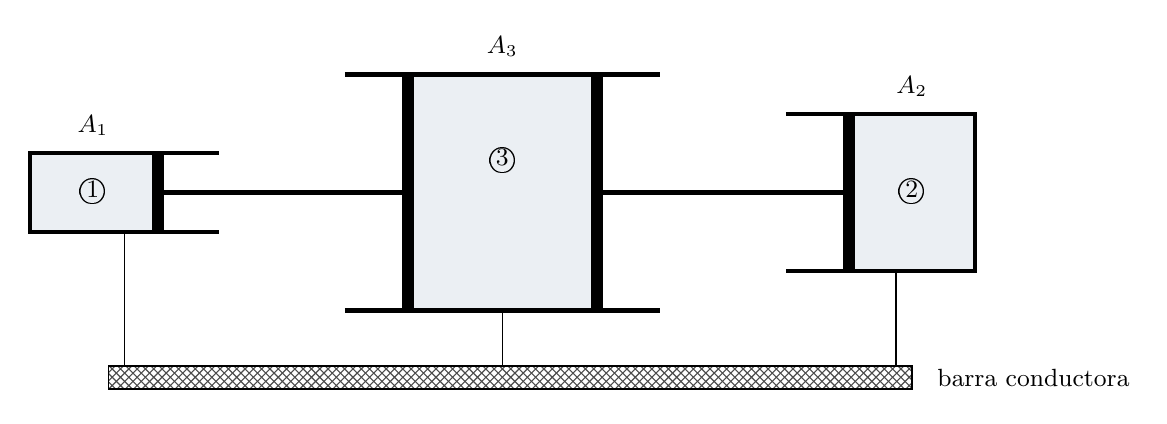
\begin{tikzpicture}
  % cilindro 1
  \fill[gas] (0,-0.5) rectangle (1.6,0.5);
  \draw[pared] (2.4,0.5) -- (0,0.5) -- (0,-0.5) -- (2.4,-0.5);
  \fill (1.55,-0.5) rectangle (1.7,0.5);
  \node at (0.8,0) {\textcircled{\small 1}};
  % cilindro 3
  \fill[gas] (4.8,-1.5) rectangle (7.2,1.5);
  \draw[pared] (4,1.5) -- (8,1.5); \draw[pared] (4,-1.5) -- (8,-1.5);
  \fill (4.73,-1.5) rectangle (4.88,1.5);
  \fill (7.13,-1.5) rectangle (7.28,1.5);
  \node at (6.0,0.4) {\textcircled{\small 3}};
  % cilindro 2
  \fill[gas] (10.4,-1) rectangle (12,1);
  \draw[pared] (9.6,1) -- (12,1) -- (12,-1) -- (9.6,-1);
  \fill (10.33,-1) rectangle (10.48,1);
  \node at (11.2,0) {\textcircled{\small 2}};
  % varillas
  \draw[line width=1.6pt] (1.7,0) -- (4.73,0);
  \draw[line width=1.6pt] (7.28,0) -- (10.33,0);
  % barra conductora de calor
  \draw[line width=0.6pt] (1.2,-0.5) -- (1.2,-2.2);
  \draw[line width=0.6pt] (6.0,-1.5) -- (6.0,-2.2);
  \draw[line width=0.6pt] (11.0,-1) -- (11.0,-2.2);
  \draw[pattern=crosshatch,pattern color=black!70,line width=0.6pt] (1.0,-2.5) rectangle (11.2,-2.2);
  \node[right] at (11.4,-2.35) {barra conductora};
  % áreas
  \node at (0.8,0.85) {$A_1$}; \node at (6.0,1.85) {$A_3$}; \node at (11.2,1.35) {$A_2$};
\end{tikzpicture}
\end{document}
